\documentclass[12pt]{article}

\usepackage{amssymb,amsmath,amsfonts,eurosym,geometry,ulem,graphicx,caption,color,setspace,sectsty,comment,footmisc,caption,pdflscape,subfigure,array,hyperref}
\usepackage{makecell}
%\usepackage{natbib}
\usepackage{apacite}
\usepackage [english]{babel}
\usepackage [autostyle, english = american]{csquotes}
\MakeOuterQuote{"}

\renewcommand\theadalign{cc}
\renewcommand\theadfont{\bfseries}
\renewcommand\theadgape{\Gape[4pt]}
\renewcommand\cellgape{\Gape[4pt]}

\normalem

\onehalfspacing
\newtheorem{theorem}{Theorem}
\newtheorem{corollary}[theorem]{Corollary}
\newtheorem{proposition}{Proposition}
\newenvironment{proof}[1][Proof]{\noindent\textbf{#1.} }{\ \rule{0.5em}{0.5em}}

\newtheorem{hyp}{Hypothesis}
\newtheorem{subhyp}{Hypothesis}[hyp]
\renewcommand{\thesubhyp}{\thehyp\alph{subhyp}}

\newcommand{\red}[1]{{\color{red} #1}}
\newcommand{\blue}[1]{{\color{blue} #1}}

\newcolumntype{L}[1]{>{\raggedright\let\newline\\arraybackslash\hspace{0pt}}m{#1}}
\newcolumntype{C}[1]{>{\centering\let\newline\\arraybackslash\hspace{0pt}}m{#1}}
\newcolumntype{R}[1]{>{\raggedleft\let\newline\\arraybackslash\hspace{0pt}}m{#1}}

\geometry{left=1.0in,right=1.0in,top=1.0in,bottom=1.0in}

\begin{document}

\begin{titlepage}
\title{Replacing the Child Tax Credit with a \protect\\Universal Child Benefit}
\author{Max Ghenis}
\date{April 2018}
\maketitle
\begin{abstract}
\noindent The Child Tax Credit is one of the largest assistance programs for children in the United States, but its structure results in smaller benefits for the poorest households. I model replacement of the Child Tax Credit with a revenue-neutral universal child benefit using data from the Current Population Survey. This would reduce inequality and child poverty, and increase after-tax after-transfer income for the bottom quartile of tax filers with children by 8 percent. A universal child benefit of \$2,000 would cost \$46 billion per year, and increase the magnitude of each effect without reducing income for any households.
\vspace{1in}\\
%\noindent\textbf{Keywords:} key1, key2, key3\\
\vspace{0in}\\
%\noindent\textbf{JEL Codes:} key1, key2, key3\\

\bigskip
\end{abstract}
\setcounter{page}{0}
\thispagestyle{empty}
\end{titlepage}
\pagebreak \newpage




\doublespacing


\section{Introduction} \label{sec:introduction}

The Child Tax Credit (CTC) is a partially refundable credit which provides a maximum of \$2,000 per child per year. However, like most tax credits, it provides little if any assistance to the poorest households. This article considers the replacement of the CTC with two versions of a universal child benefit: a \$1,450\footnote{Based on CPS data.} payment and a \$2,000 payment. The former is revenue-neutral, while the latter avoids any families losing income after taxes and transfers.

By reaching the poorest families who are often ineligible and/or do not file taxes to receive the CTC, both reforms reduce child poverty (using three different measures) and inequality (using the Gini index). Studies on child cash transfers suggest that this child poverty reduction would improve children's health, education, and earnings.

I begin by summarizing the CTC, other countries' child benefits, US child benefit proposals, and research on cash transfers for families with children. I then describe the data and software used to model policy reforms transforming the CTC into a universal child benefit. I quantify the impact across distributions of baseline income, and for inequality and child poverty, and conclude with other potential reforms and ways to generate more robust estimates.


\section{Background} \label{sec:literature}

\subsection{The US Child Tax Credit}

The US Child Tax Credit (CTC) was created in 1997 to assist families with children under age 17. It originated as a nonrefundable credit, and has always phased out for filers above a certain income. The CTC has since grown, both in nominal value and in partial refundability, making it accessible to low-income filers \cite{crandall-hollick}. The maximum value per child increased from \$1,000 to \$2,000 as part of the Tax Cuts and Jobs Act of 2017 (TCJA), which also raised the income thresholds before the credit phases out.

\subsection{Child benefits}

Child benefits, also called child allowances, are payments made from the government to families with children.

\subsubsection{Child benefits in other countries}

Many European countries, as well as Canada, Japan, South Korea, and Australia \cite{wikipedia_child_benefit}, have some sort of child benefit, though they typically vary by family income and size. Ireland and Sweden have flat universal payments, giving families the equivalent of \$2,070 and \$1,540 tax-free per child under 16 per year, respectively \cite{citizensinformation,sweden_child_allowance}. Canada's child benefit was also universal (though taxable) until it became means-tested in 2016.

\subsubsection{US child benefit proposals}

Child poverty scholars have proposed child benefits in the US, with recent analyses comparing against the Child Tax Credit. As these analyses use data preceding the TCJA, they understate the budgetary impact of the CTC, and include child exemptions repealed in the TCJA.

\citeA{hammond2016toward} propose a \$2,000 per year child benefit, with the same phase-out as the 2016 CTC. They estimate this would cost \$143 billion, just under the combined budgets of the CTC, child exemption, child receipts for the Supplemental Nutrition Assistance Program (SNAP, formerly food stamps), and school nutrition programs. They do not perform a distributional analysis to identify "winners and losers."

\citeA{shaefer2018universal} find that a \$3,000 taxable child benefit would reduce child poverty (as defined by the Supplemental Poverty Measure) from 16.1 percent to 9.7 percent. Pairing the benefit with elimination of the CTC and child exemption would cost \$93 billion, providing a net gain to all household income groups, especially those under \$50,000. They model two modifications: first, giving children under six years old an additional \$50 per month, following Hillary Clinton's 2016 proposal to expand the CTC for children under five years old \cite{sawhill}. Second, they consider a smaller amount per child for families with multiple children, by applying the formula $BenefitAmount * NumberOfChildren^{0.7}$. They propose distributing the payment monthly to address higher intra-year income volatility among low-income families.

\citeA{bitler2018cash} calculates that a universal child benefit of approximately \$2,000 could replace several child-oriented programs: the Child Tax Credit; the now-defunct child exemption; and child-related parts of the Earned Income Tax Credit (EITC). This revenue-neutral plan would provide a significant net gain for families under 75 percent of the poverty line, a net loss for those between 75 and 200 percent of the poverty line (who benefited most from the CTC and EITC), and a smaller net gain for families over 200 percent of the poverty line.

\subsection{Effects of cash transfers on children}

Experimental and quasi-experimental evidence from the US and other countries shows that cash transfers for families have positive effects on children. 

The quasi-experimental literature has leveraged variation in income resulting from program changes. \citeA{dahl2012impact} exploit changes to the EITC to find that "a \$1,000 increase in income raises combined math and reading test scores by 6 percent of a standard deviation in the short run." \citeA{nichols2015earned} review several other studies on EITC's positive effects, while noting that increased labor force participation could also explain results, given the EITC also (by design) increases labor supply. \citeA{milligan2011child} study changes in Canada's child benefit, finding that "child benefit programs had significant positive effects on test scores, maternal health, and mental health." 

Comparing results from different welfare-reform experiments in the 1990s, \citeA{duncan2011does} find that a \$1,000 increase in family income increases children's achievement test scores by around 5 percent of a standard deviation.

Studies from developing countries provide a large body of evidence for cash transfers, including experimental evidence using randomized controlled trials, as summarized by \citeA{givedirectly} across 14 studies: "Many studies find positive effects on the health of children—for example, large increases in height-for-age and weight-for-height in South Africa, large reductions in HIV infection rates and psychological distress in Malawi, and large reductions in the incidence of low birth weight in Uruguay. Several studies also find that unconditional cash transfers (UCTs) substantially increase schooling and decrease child labor."

\section{Data} \label{sec:data}

I use data from the 2014 Current Population Survey (CPS) as processed and projected to 2018 by the Tax-Calculator software \cite{using_taxcalc}\footnote{Tax-Calculator forms CPS household records into 456,465 tax filing units, assigns them weights to minimize error against target totals (for example total income tax), and adjusts weights each year to project data for the 2018 tax year.}. I restrict all analysis to tax units with at least one child eligible for the CTC (hereafter "child").

The primary metric used is the tax unit's income after taxes and transfers (hereafter "income"). Both cash and in-kind transfers are based on the CPS Annual Social and Economic Supplement (ASEC), and adjusted for systematic underreporting using the CPS Transfer Augmentation Model (C-TAM)\footnote{Transfer programs include Medicaid; Medicare; Supplemental Security Income; Supplemental Nutritional Assistance Program; Veterans Benefits; Social Security; Housing Assistance; Unemployment Insurance; Temporary Assistance for Needy Families; Workman's Compensation; Special Supplemental Nutrition Program for Women, Infants and Children; Affordable Care Act Premium Tax Credit; and other smaller programs.}.

Tax-Calculator provides both data and modeling. I model elimination of the Child Tax Credit by setting the value of the CTC and child dependent credit (introduced in the TCJA as a complement to the core CTC) to zero using Tax-Calculator's Python interface. Since the CTC has a minor effect on other tax elements, I report the effect on total income, as opposed to only the value of the credit. This modeling yields a dataset with each tax unit's income, income without the CTC, number of children, number of people, and weight.

As of the version used here (0.18.0), Tax-Calculator CPS data contains errors that affect this analysis, in particular including 17-year-olds in the set of CTC-eligible children and overestimating the total number of children. Other known issues are logged in the Tax-Calculator, taxdata, and C-TAM GitHub repositories \cite{open_source_economics}.

For these reasons and for robustness checks, some results are estimated using an alternative Tax-Calculator dataset: the Public Use File (PUF). This is a sample of tax records sold by the Internal Revenue Service.

This analysis is produced from two Jupyter \cite{Kluyver:2016aa} notebooks: one using the CPS data \cite{ghenis_notebook} and one using the PUF data \cite{ghenis_puf_notebook}.

\section{Results} \label{sec:result}

\subsection{CTC budgetary impact}

A revenue-neutral child benefit is calculated as the CTC's budgetary impact divided by the number of eligible children. Tax-Calculator produces different estimates for each metric depending on whether CPS or PUF data is used. As an external comparison point for the budgetary impact, we can add the Tax Policy Center's (TPC) 2017 estimate of the budgetary impact with the Joint Committee on Taxation's (JCT) estimate of the CTC expansion's impact for the 2019 budget; these are \$52 billion \cite{maag} and \$68 billion \cite{jct}, respectively.\footnote{This assumes no "organic" cost differences between the 2017 and 2019.} Table \ref{table:ctcbudget} shows this information, as well as the Census estimate of children under 17 years old \cite{ghenis_pop_tc_vs_census}.

% Currently needed as they aren't attached.
\pagebreak \newpage

\begin{center}
\captionof{table}{CTC budgetary impact and children by dataset}
\begin{tabular}{p{4cm}p{3.5cm}p{3.5cm}p{3.5cm}}
 \thead{Dataset} & \thead{CTC budgetary \\ impact} & \thead{CTC-eligible \\ children} & \thead{CTC budgetary \\impact per \\eligible child} \\ [0.5ex] 
 \hline
 Tax-Calculator (CPS) & \$124 billion & 85.1 million & \$1,457 \\ 
 \hline
 Tax-Calculator (PUF) & \$114 billion & 70.0 million & \$1,621 \\
 \hline
 TPC/JCT/Census & \$120 billion & 69.4 million & \$1,729 \\ [1ex] 
 \hline
\end{tabular}
\label{table:ctcbudget}
\end{center}

While the CPS data aligns more closely with the TPC/JCT budgetary impact estimate (3 percent vs. 5 percent), the PUF aligns much more closely on both the number of children (1 percent vs. 22 percent) and budgetary impact per child (6 percent vs. 16 percent).

Nevertheless, it's unclear whether the CPS data significantly misrepresents the distributional impact of policy reforms. Since it is publicly available and therefore reproducible, this article reports CPS-based results unless otherwise specified.

\subsection{CTC benefits before and after TCJA}

Rather than consider the complex rules governing the CTC's refundability, phase-in, and phase-out, we can examine distribution of outcomes to understand the credit's benefit. Figure \ref{fig:avg_ctc_per_child} shows the average credit value per child based on the household's income percentile without the credit.

\begin{center}
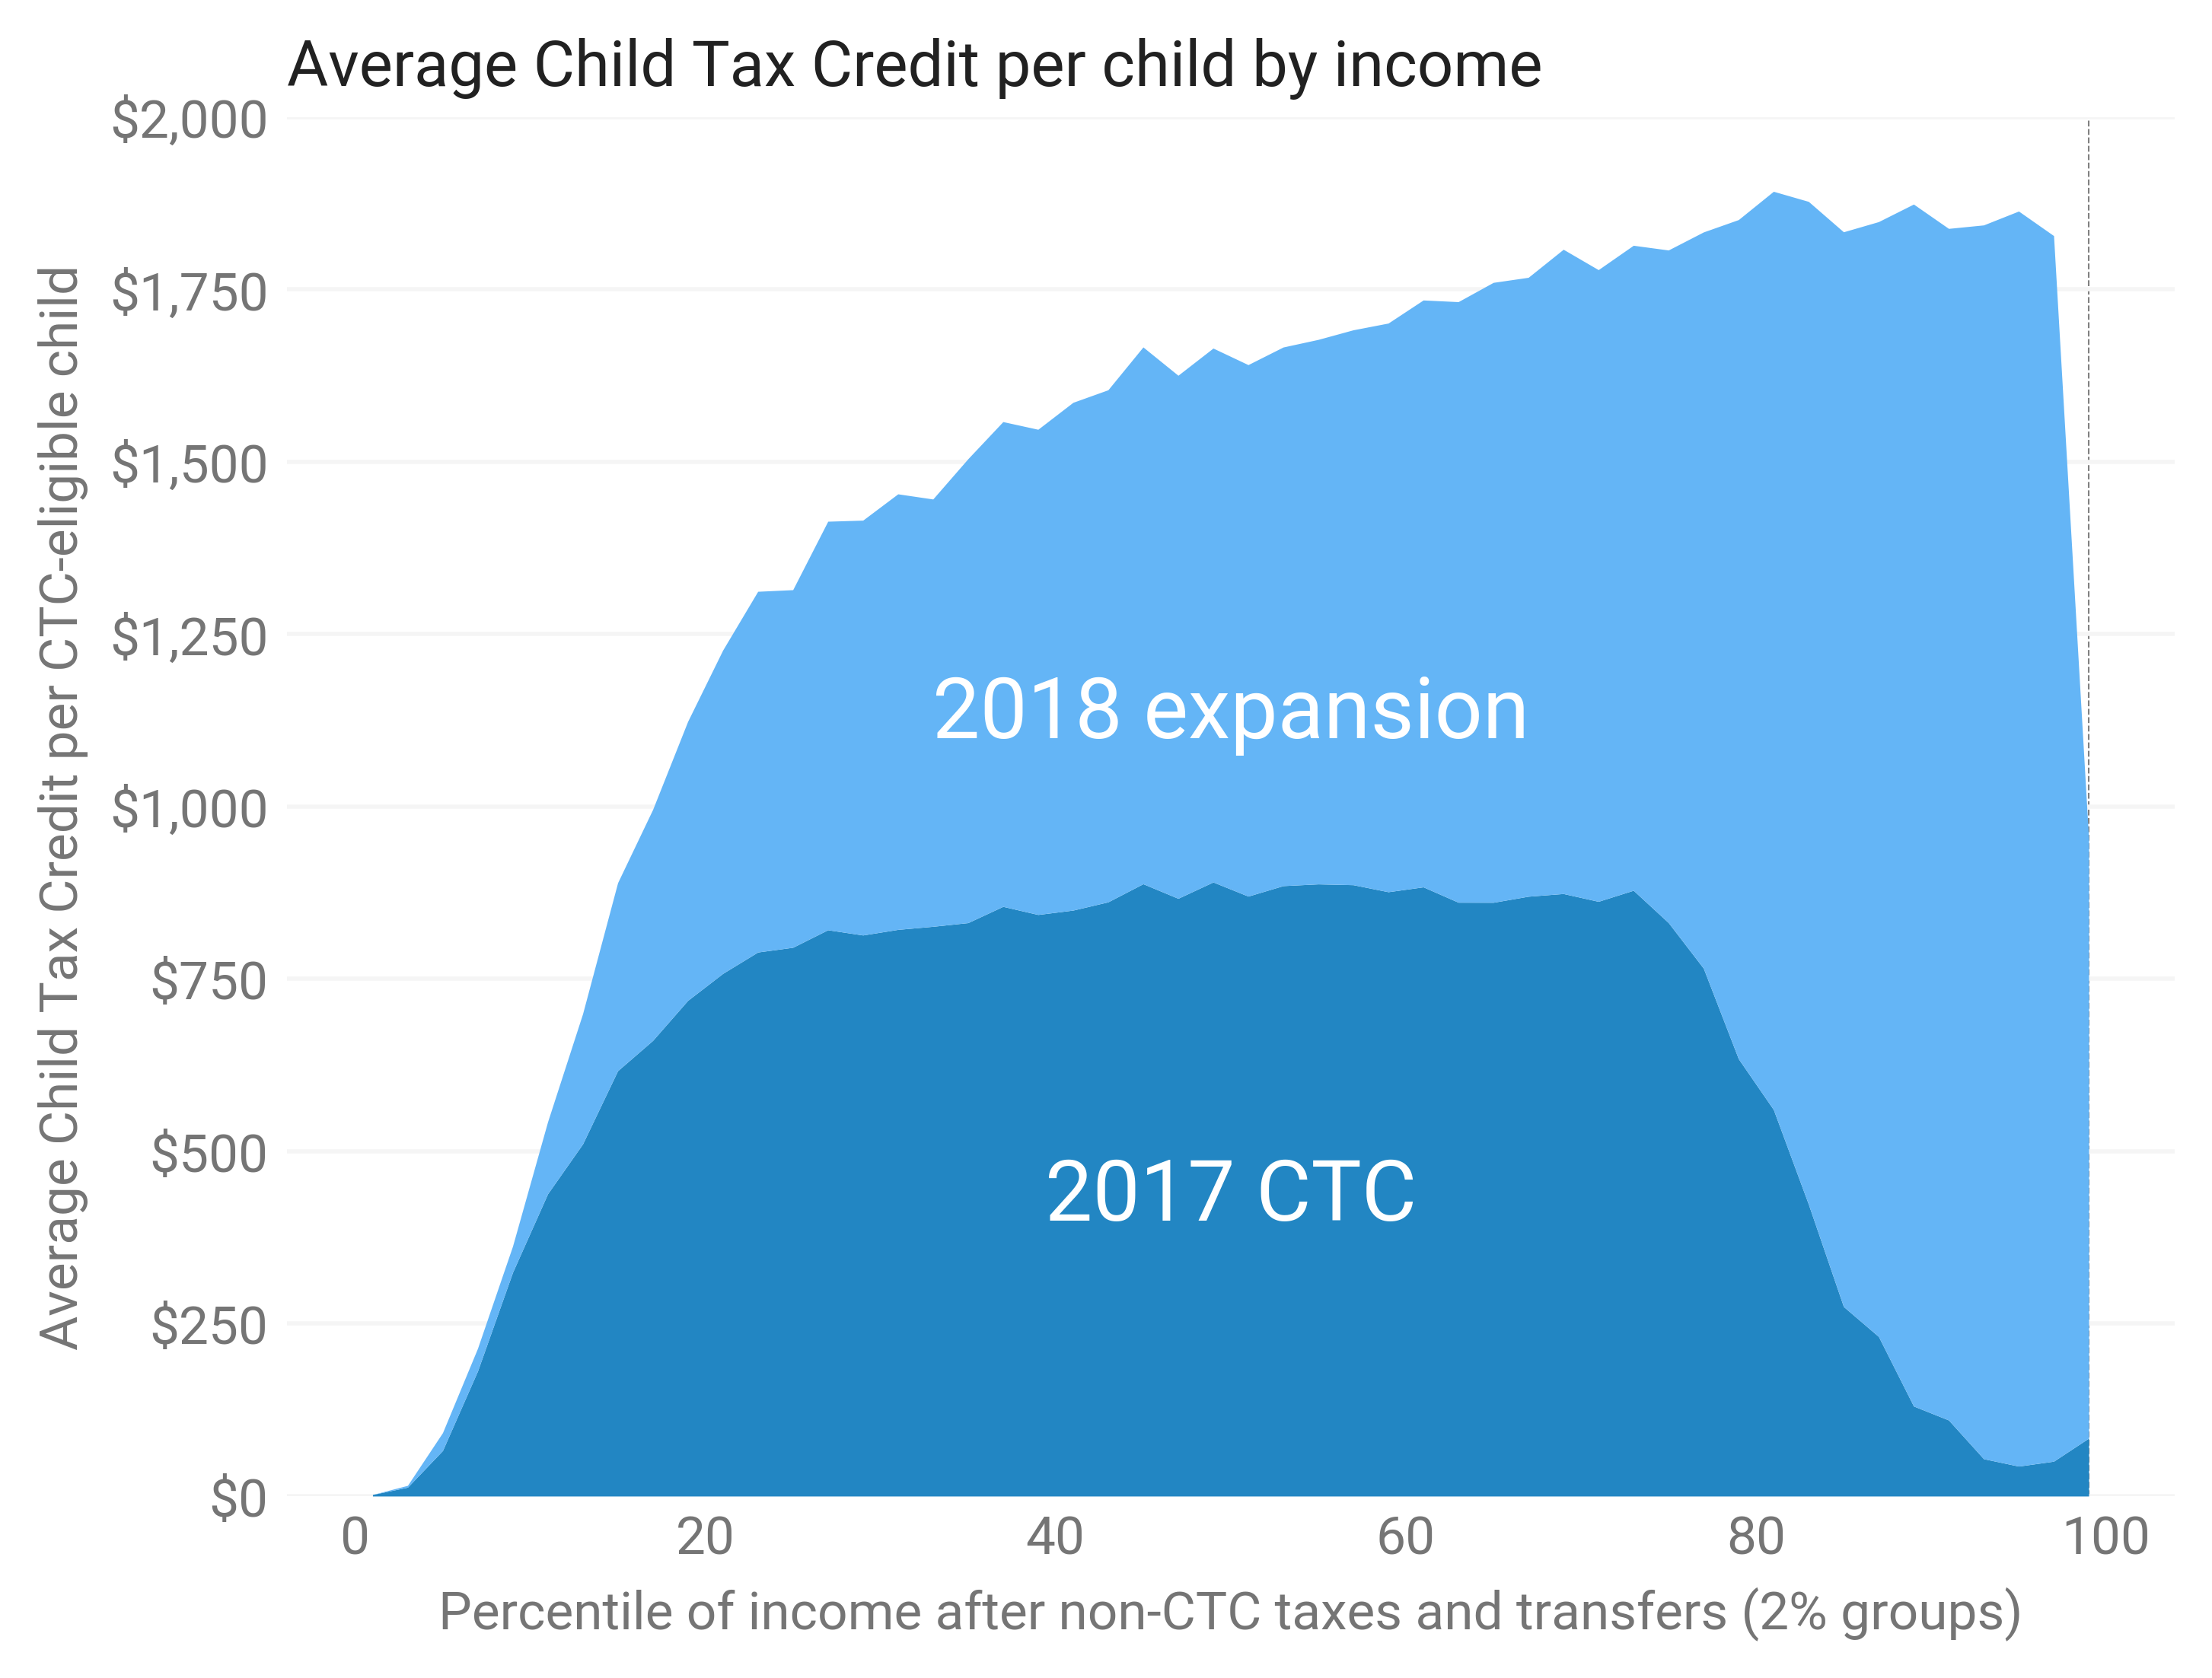
\includegraphics[width=15cm]{avg_ctc_per_child.png}
\captionof{figure}{}
\label{fig:avg_ctc_per_child}
\end{center}

The average credit per child exceeds \$1,500 for most percentiles outside the bottom third, up until the top 1 to 2 percent who are ineligible. While the TCJA disproportionately helped upper-middle income families,\footnote{Part of this is offset by elimination of child exemptions, which disproportionately helped higher earners due to them having higher marginal tax rates.} it did not benefit very low earners who already had smaller benefits.

\subsection{Replacing the CTC with a universal child benefit}

Dividing the \$124 billion budgetary impact of the CTC by the 85.1 million children would yield \$1,457 per child. This would then be the value of a revenue-neutral child benefit, which we hereafter round to \$1,450. Increasing the benefit to \$2,000 per child would cost \$46 billion (\$27 billion using PUF data).

\subsubsection{Distributional impact}

Replacing the CTC with a \$1,450 revenue-neutral child benefit would raise by 7.6 percent the income of the bottom quartile, while reducing it by 0.5 percent for the remainder of filers. Replacing it with a \$2,000 child benefit would raise the bottom quartile's incomes by 13 percent, and also raise the income for other tax units by 0.6 percent. While the revenue-neutral plan has a relatively constant effect across the upper three quartiles, the \$2,000 benefit would be progressive at each quartile (see Figure \ref{fig:quartiles}).

\begin{center}
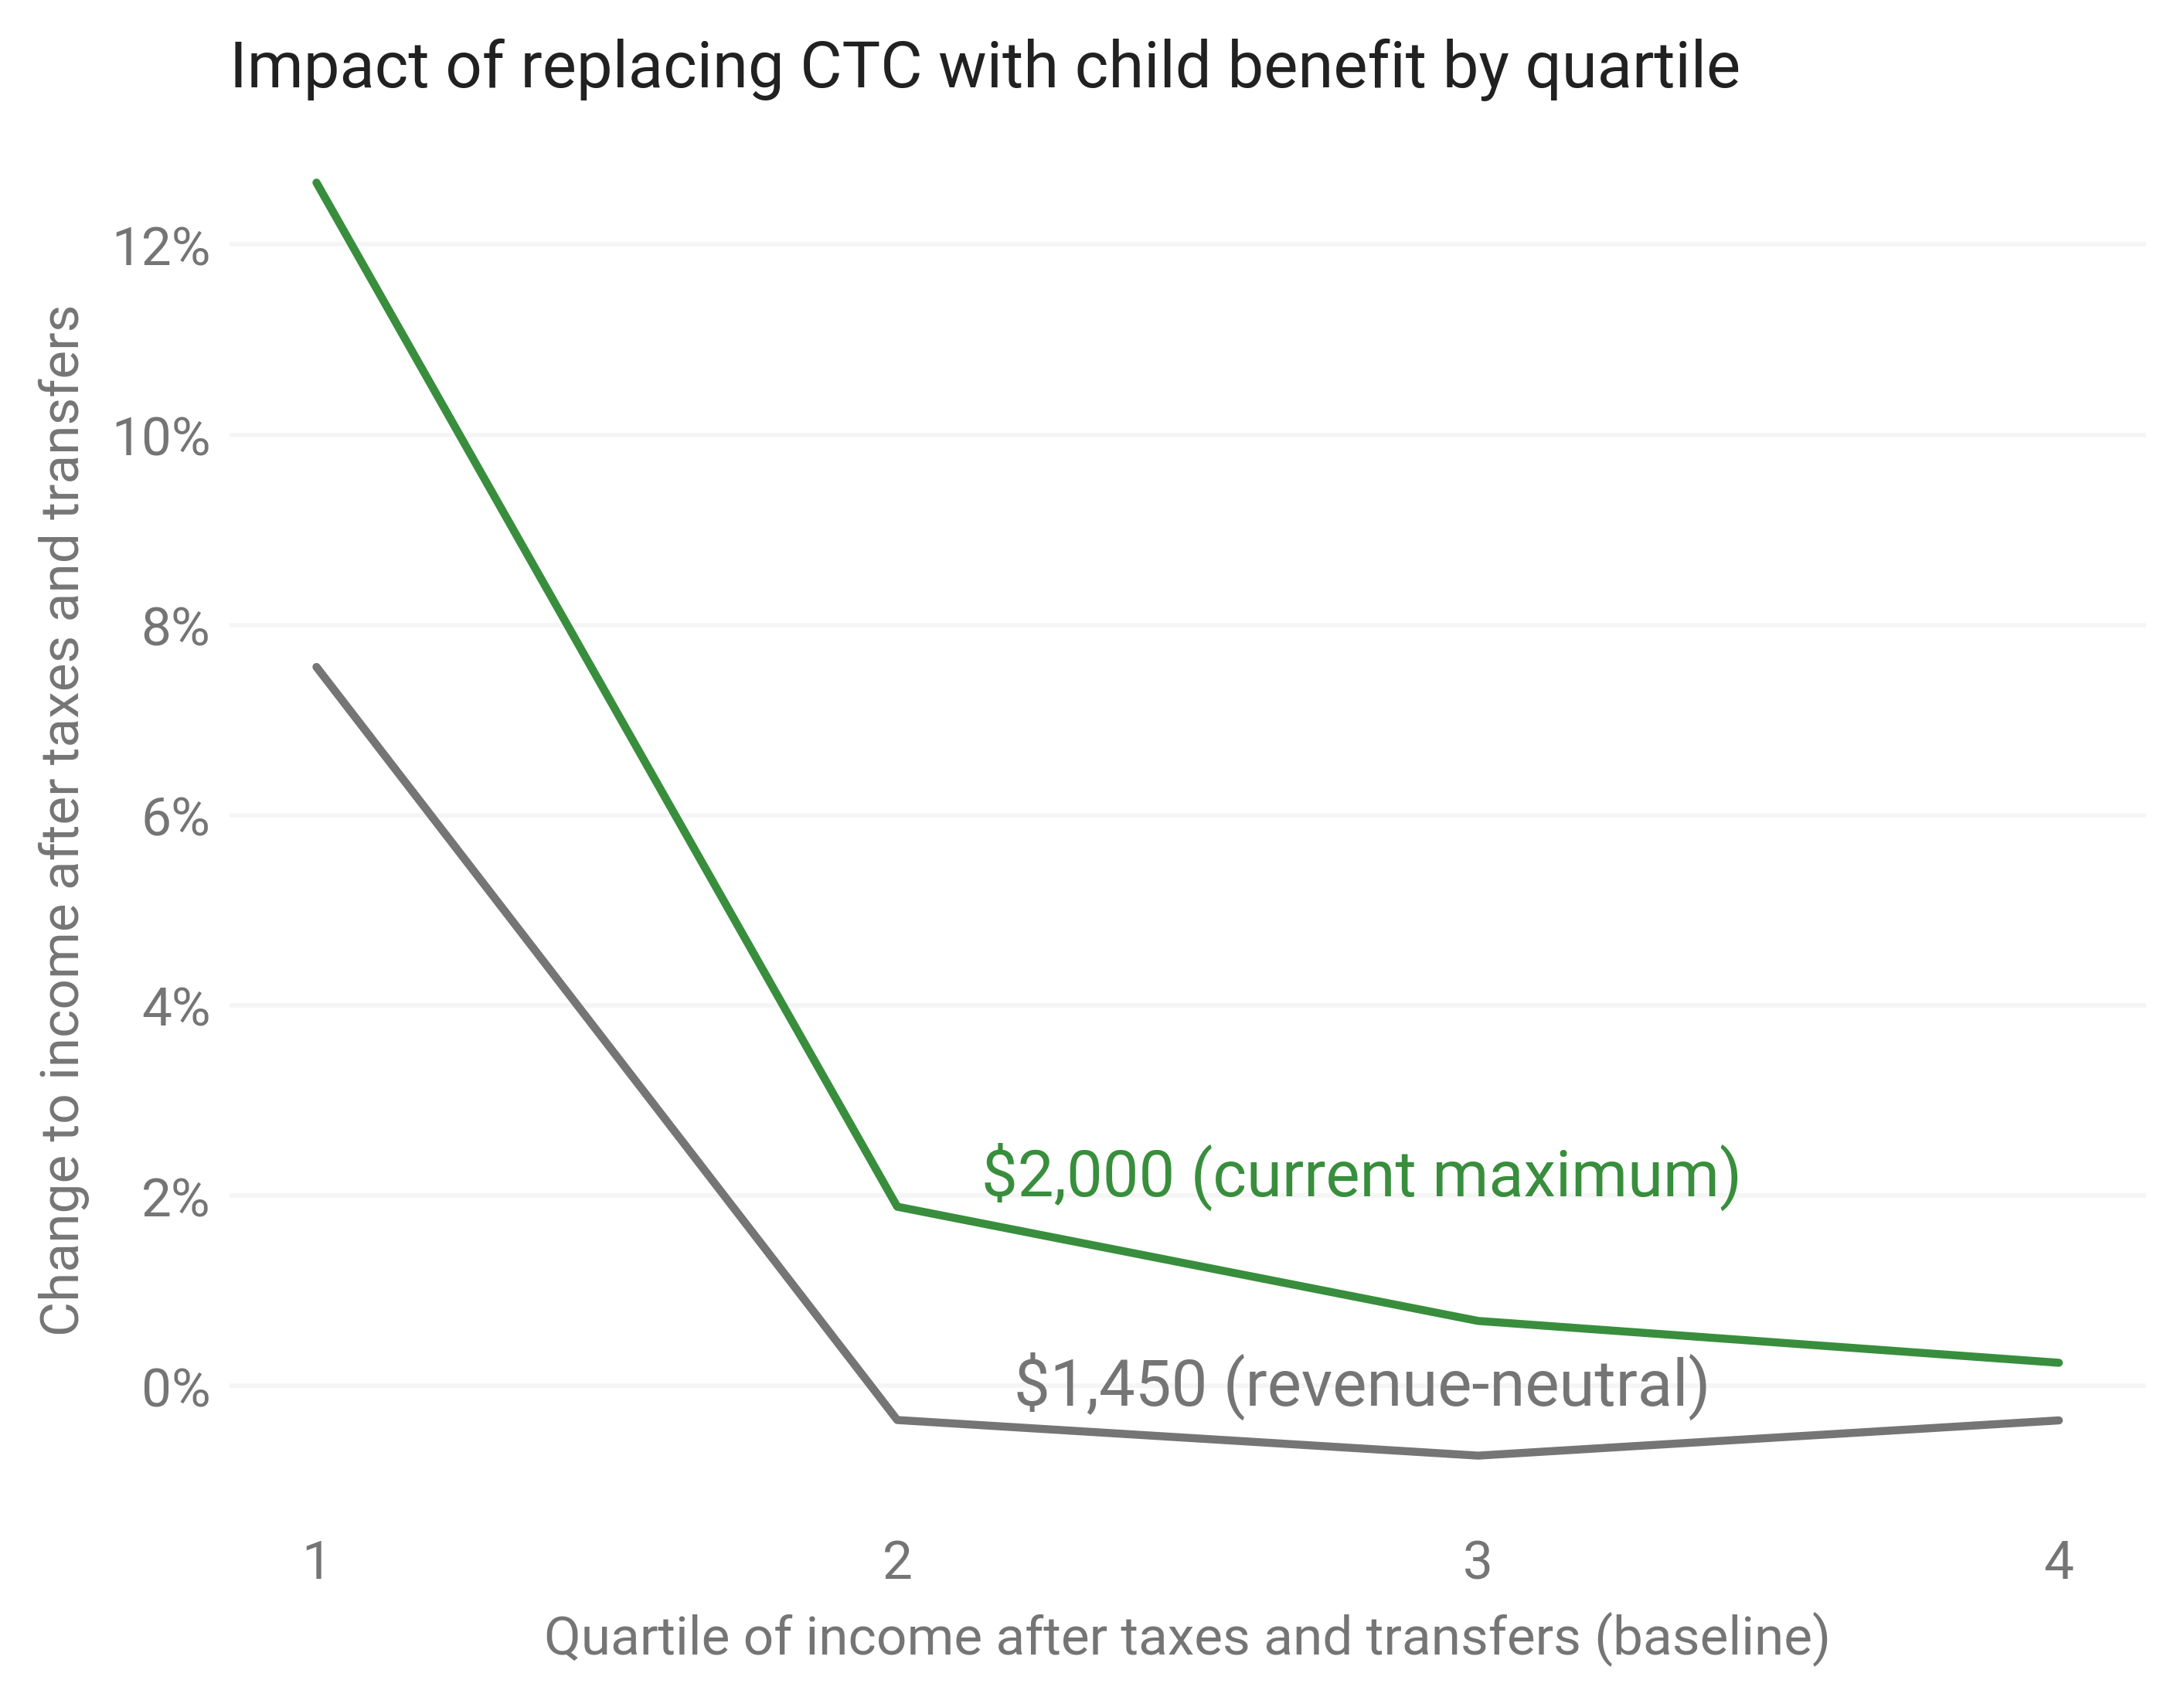
\includegraphics[width=15cm]{quartiles.png}
\captionof{figure}{}
\label{fig:quartiles}
\end{center}

Zooming in on the bottom quartile in Figure \ref{fig:bottom_quartile} shows that the bottom 5 percent increase their incomes by 145 percent under the revenue-neutral plan and 200 percent in the \$2,000 plan. This group has an average income of \$2.90 per person per day, though extremes of the income distribution are difficult to measure \cite{ghenis_bottom_income}.

\begin{center}
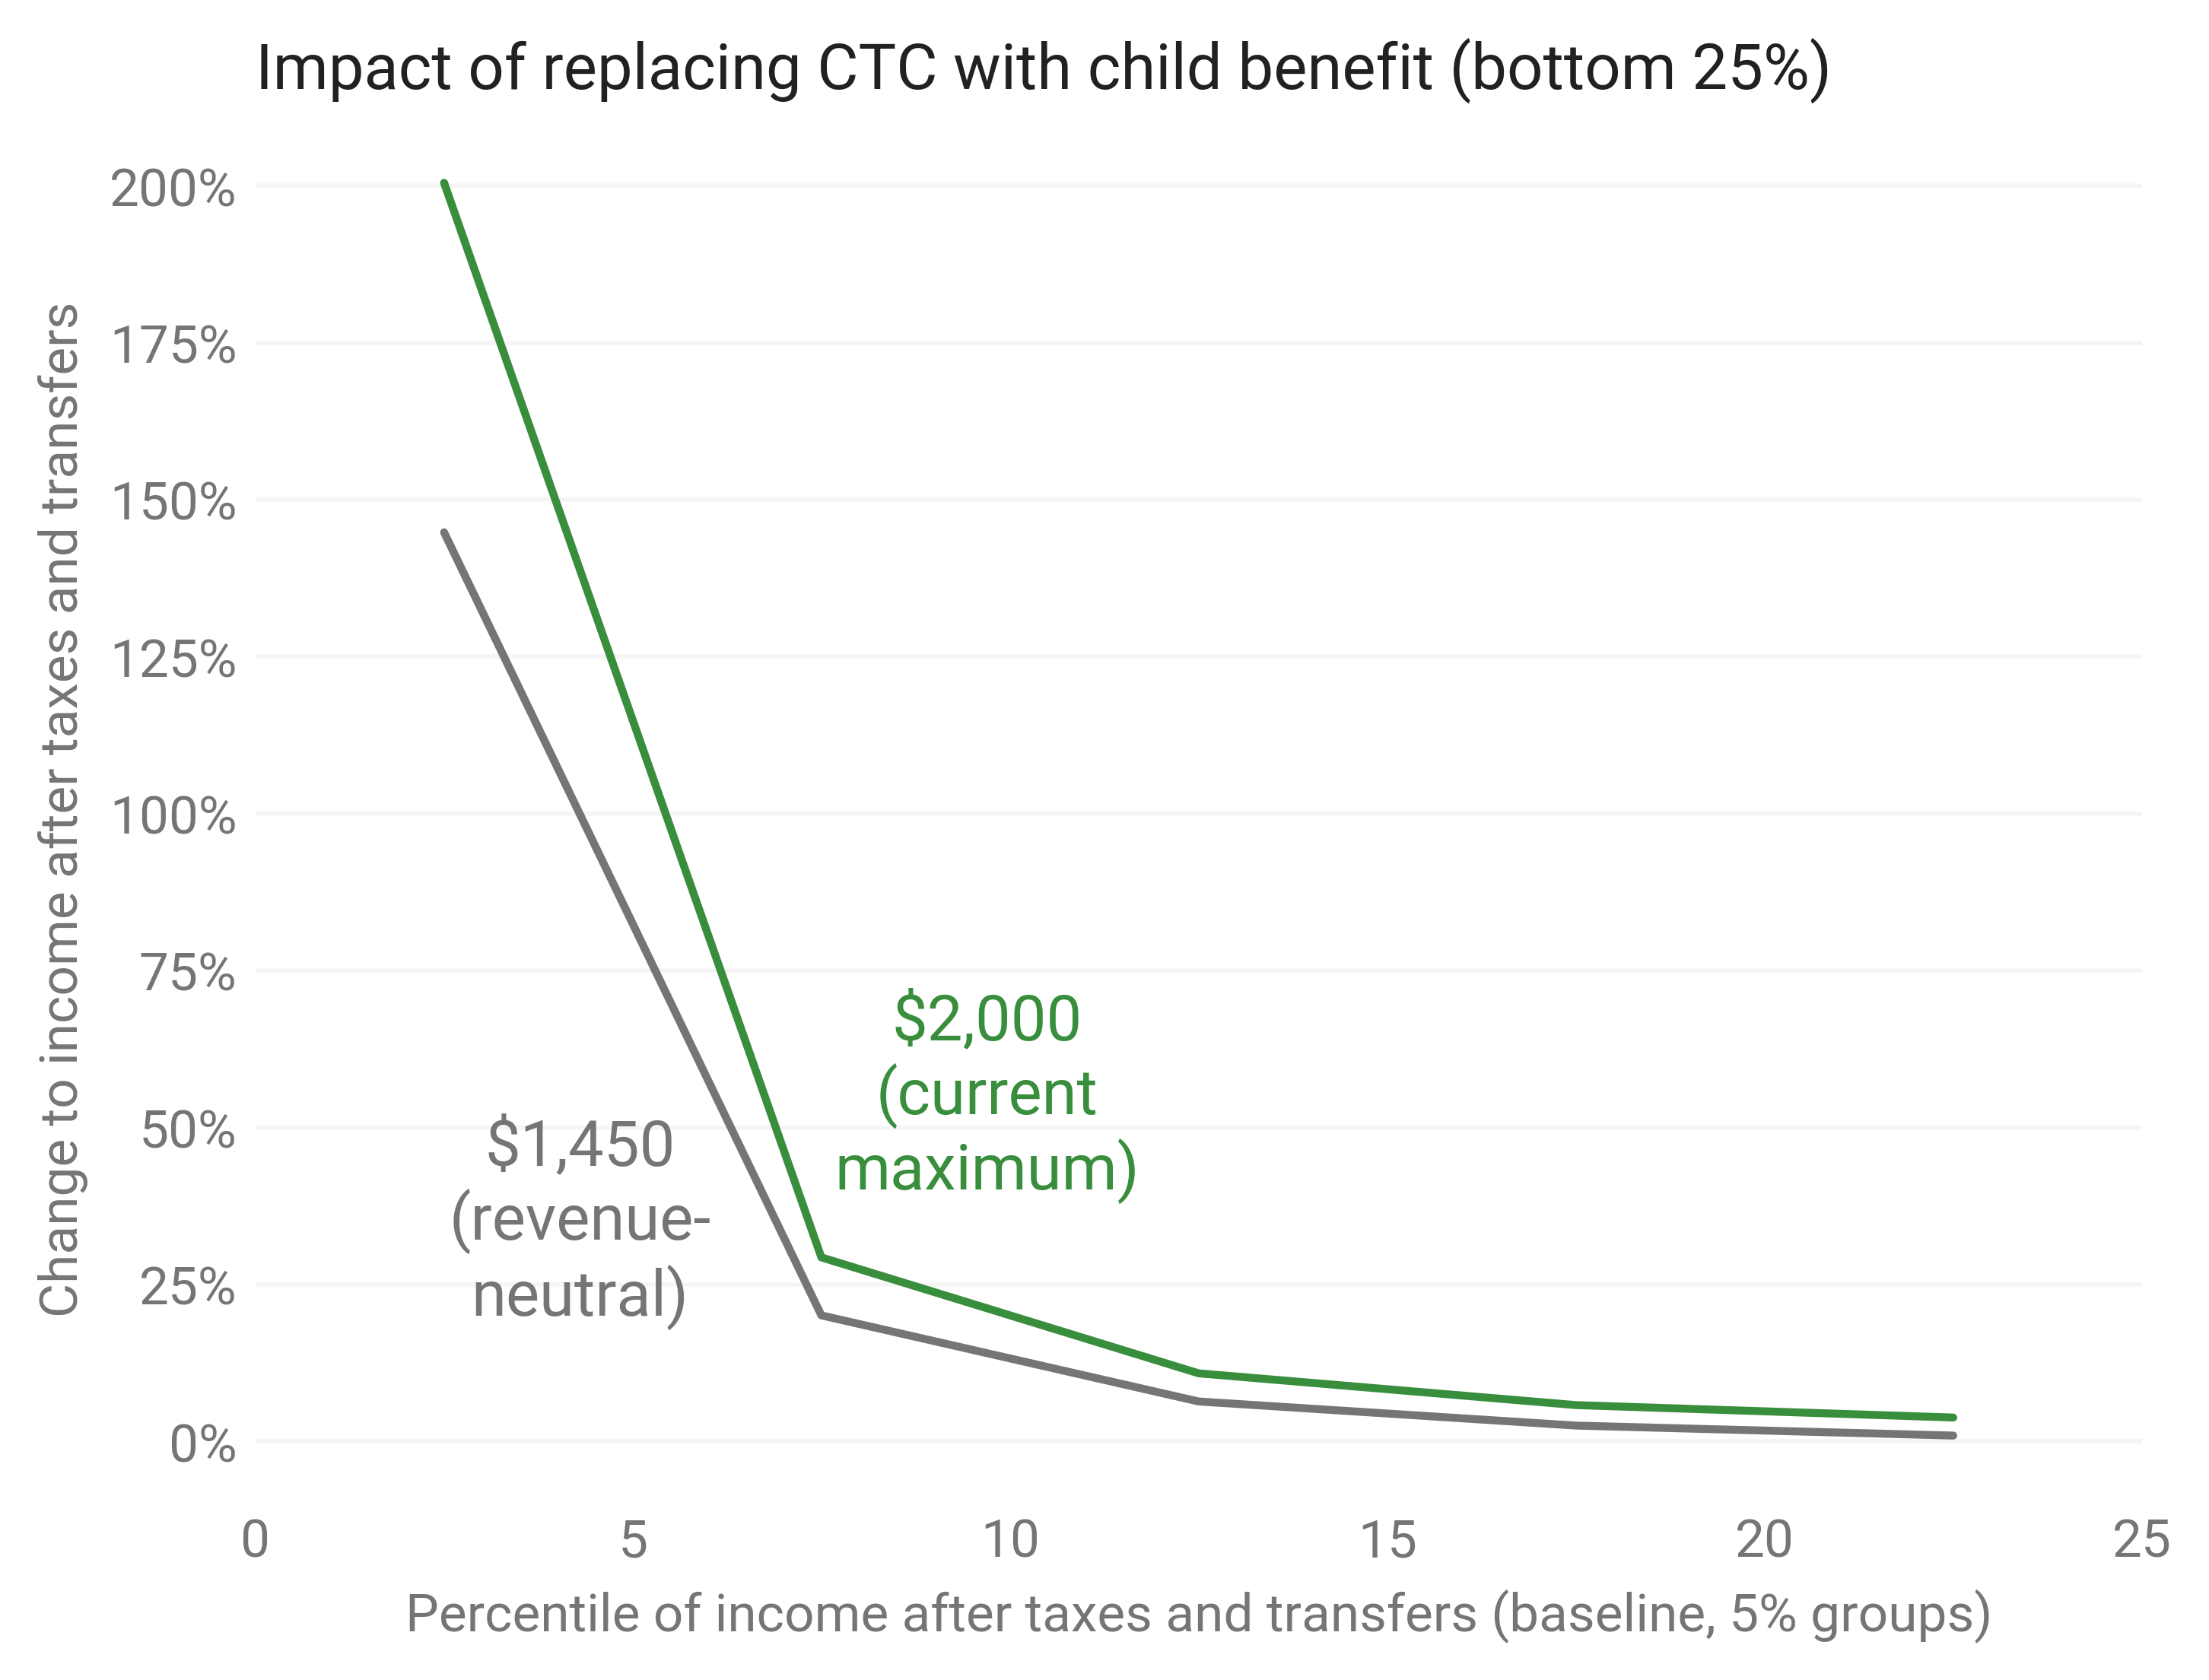
\includegraphics[width=15cm]{bottom_quartile.png}
\captionof{figure}{}
\label{fig:bottom_quartile}
\end{center}

The universal child benefit results in higher incomes for the top two percent of filers with children (Figure \ref{fig:upper_75p}): 0.20 percent higher in the revenue-neutral plan, and 0.41 percent higher in the \$2,000 plan. This follows from the current CTC phasing out for filers with incomes above \$200,000, or \$400,000 if filing jointly.

\begin{center}
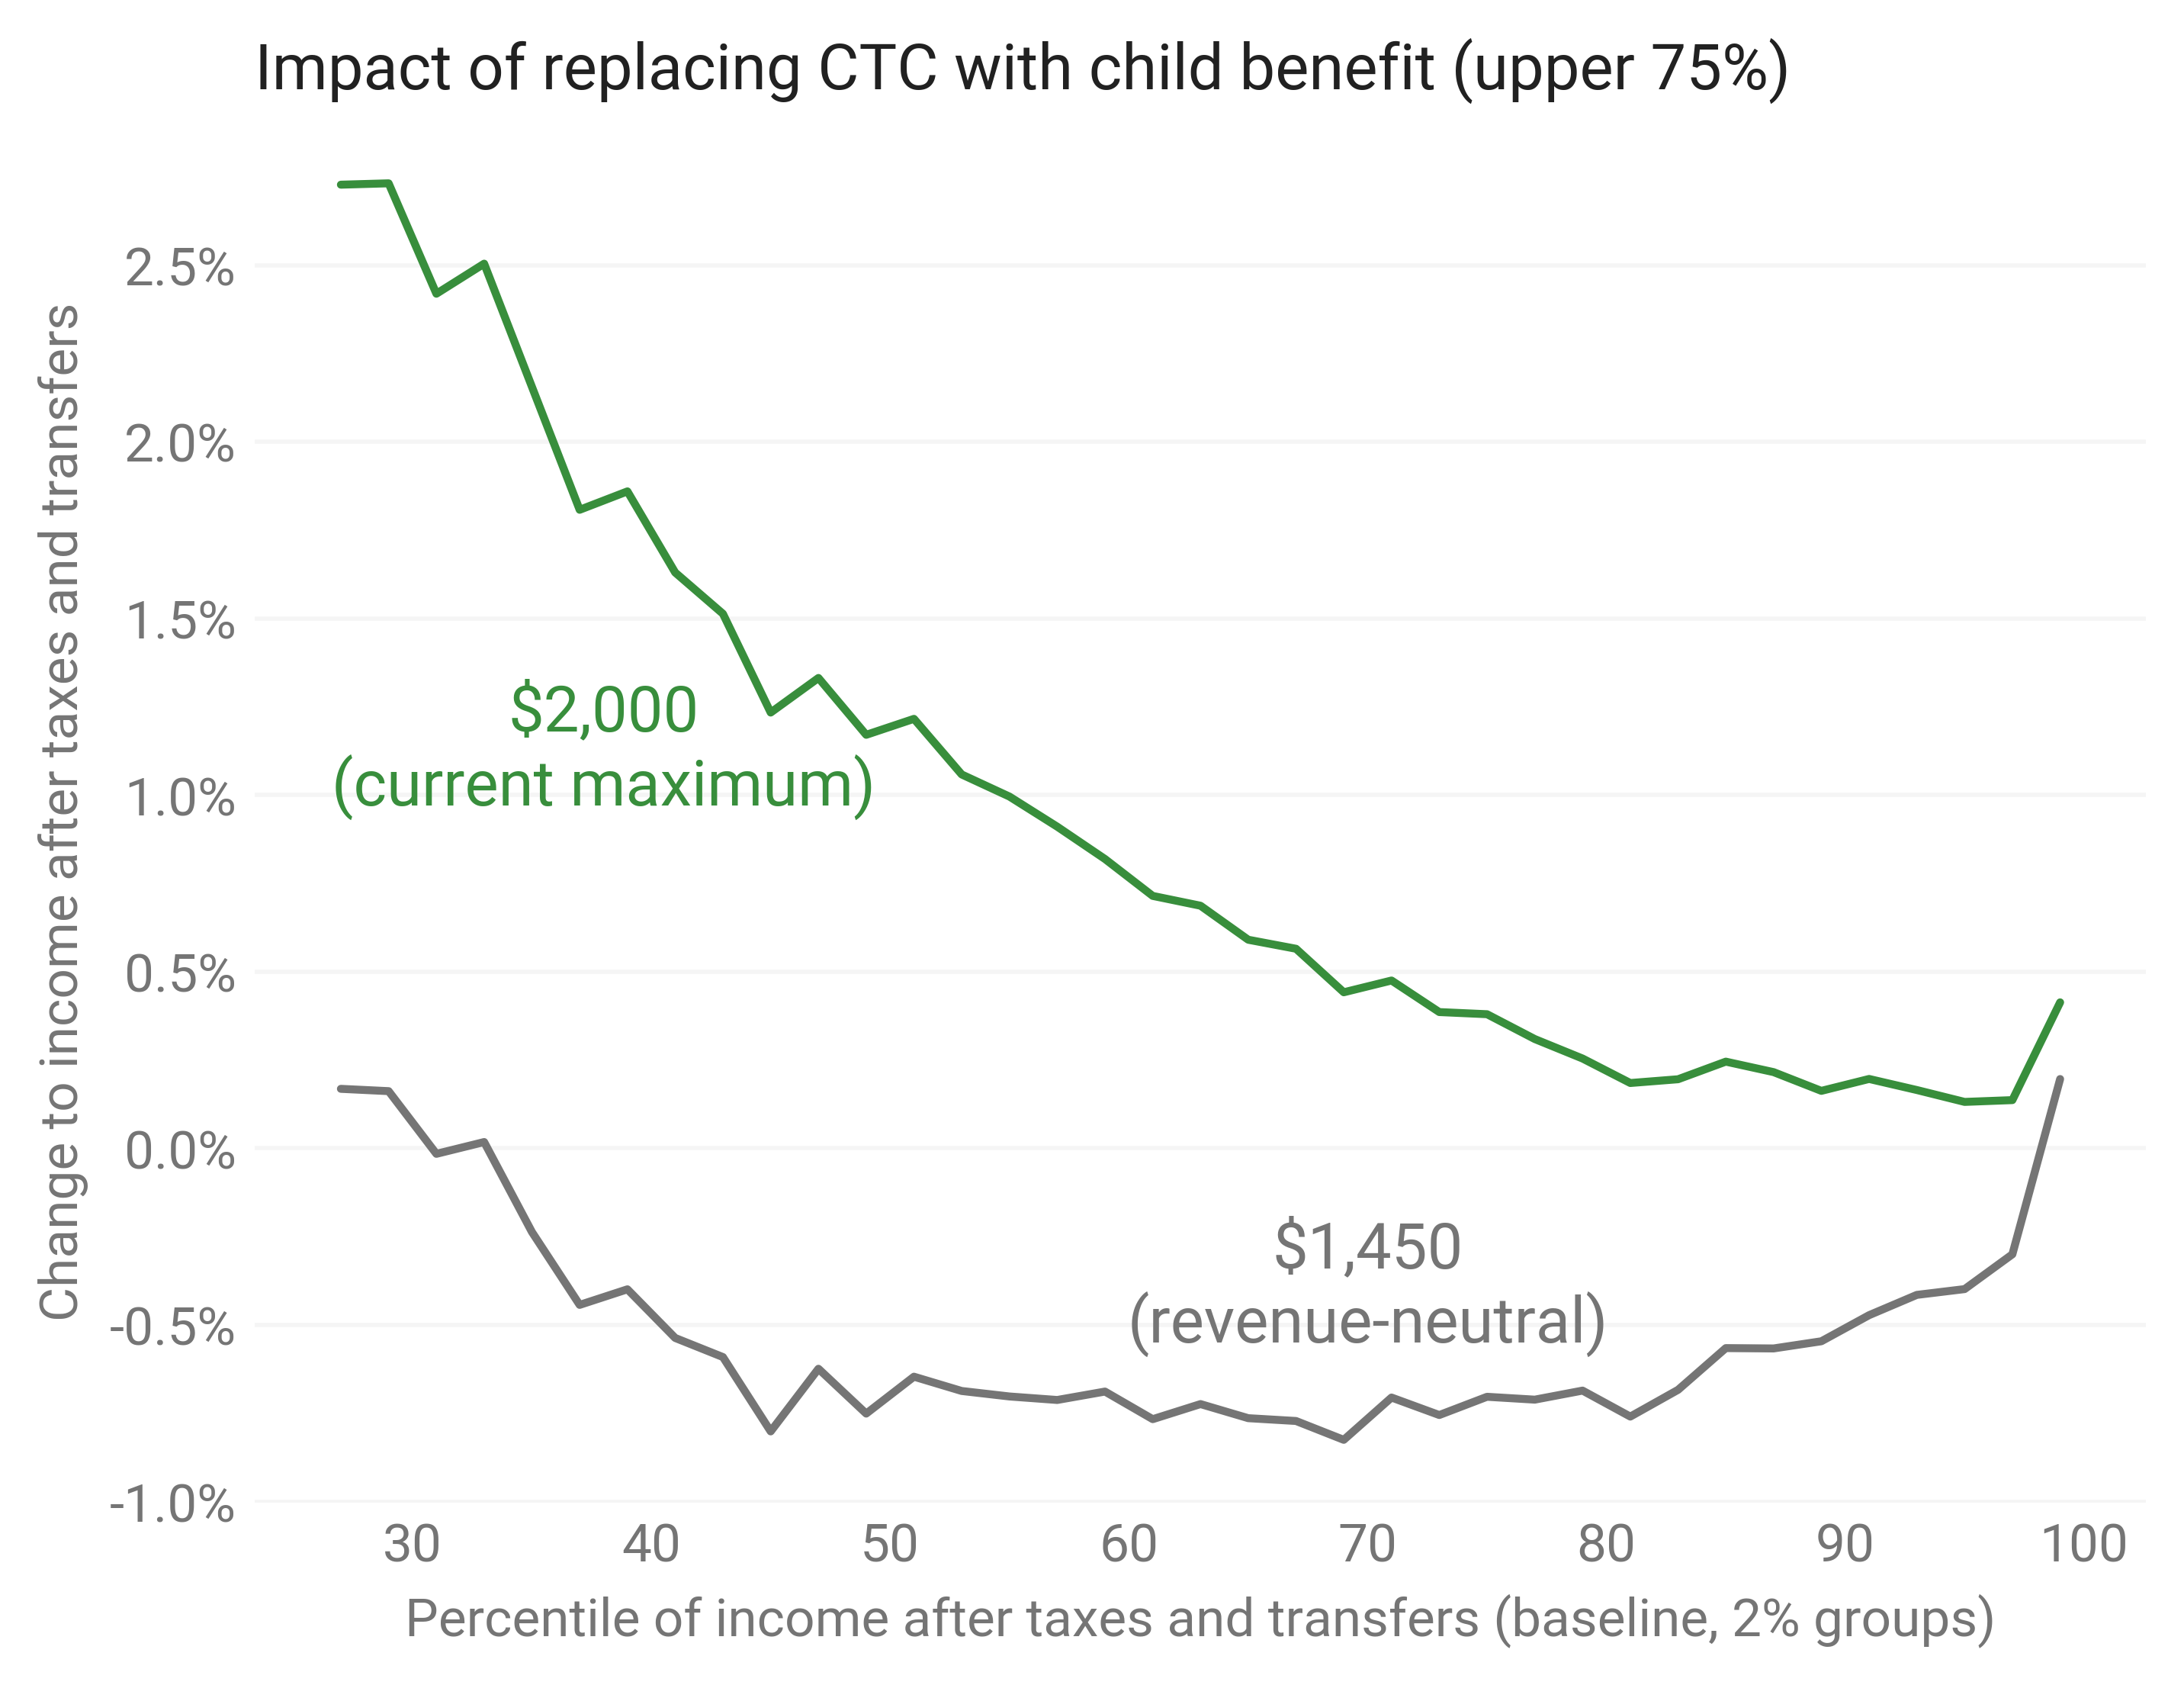
\includegraphics[width=15cm]{upper_75p.png}
\captionof{figure}{}
\label{fig:upper_75p}
\end{center}

Both reforms reduce inequality, as measured by the Gini coefficient. This measure lies between 0 (perfect equality) and 1 (perfect inequality), and is currently 0.458 among US filers with children. The revenue-neutral plan would reduce it to 0.453, while the \$2,000 plan would reduce it to 0.448.

\subsubsection{Impact on child poverty}

Estimating the effect of a child benefit on child poverty requires a metric that incorporates taxes and transfers, and which the Tax-Calculator income data supports. As Table \ref{table:poverty_measures} shows, this rules out four commonly used measures of child poverty.

\clearpage
% Ideally tie the caption to the table.

\begin{center}
\captionof{table}{Poverty measure data availability}
\begin{tabular}{p{2.5cm}p{8cm}p{3cm}p{2.5cm}}
 \thead{Measure} & \thead{Description} & \thead{US estimate} & \thead{Obstacles} \\ [0.5ex]
 \hline
 {\footnotesize Extreme poverty} & {\scriptsize \citeA{wb_poverty} defines for international comparisons as consumption \cite{roser} below \$1.90 per day per person, in 2011 dollars adjusted for purchasing power. This is about \$780 in 2018 dollars per person per year in the US.} & {\scriptsize Under 0.1 percent of all persons as of 2011 \cite{chandy2014poor}. No child-specific data available.} & {\scriptsize Tax-Calculator data measures income, not consumption.} \\ 
 \hline
 {\footnotesize US poverty threshold} & {\scriptsize \citeA{census_poverty_thresholds} defines for poverty reporting. Based on the number and age of household members, and only includes earnings and cash transfers (not taxes, tax credits, or in-kind transfers). The 2017 threshold for a household with one person under age 65 and one child was \$16,895.} & {\scriptsize 21 percent of children \cite{nccp} (no year specified).} & {\scriptsize While this would count the child benefit, it does not count the CTC.} \\
 \hline
 {\footnotesize US poverty guideline (federal poverty line, or FPL)} & {\scriptsize \citeA{aspe} defines for program eligibility (e.g., Medicaid). Like the poverty threshold, it is based on pre-tax cash alone, but it does not depend on age. For the contiguous states, the FPL is \$12,140 for a household with one person, plus \$4,320 for each additional person.} & {\scriptsize None found.} & {\scriptsize Same as poverty threshold.} \\
 \hline
 {\footnotesize US Supplemental Poverty Measure (SPM)} & {\scriptsize U.S. Census Bureau defines for more robust poverty measurement. Includes taxes and transfers--cash and in-kind--and is adjusted based on local cost of living\cite{short2015supplemental}}. & {\scriptsize 15.6 percent of children as of 2016 \cite{shapiro2017child}.} & {\scriptsize Insufficient geographic granularity to adjust for cost of living.} \\ [1ex] 
 \hline
\label{table:poverty_measures}
\end{tabular}
\end{center}

\clearpage

Instead, I use these three measures:
\begin{enumerate}
\item Extreme poverty by income, at the same \$780 defined by the World Bank, using income rather than consumption.
\item Federal poverty line (FPL) including taxes and transfers, using levels defined for the contiguous states.
\item \$10,000 per person per year, as a simple threshold.
\end{enumerate}

By all three measures, both the revenue-neutral and \$2,000 child benefit reduce the share of children in impoverished tax units (Figure \ref{fig:poverty}). The impact is most significant for the extreme poverty measure, which falls from 1.9 percent to 0.4 and 0.2 percent for the two respective plans. Using the FPL, the child poverty rate falls by 14 percent and 22 percent, respectively, and it falls by 5 percent and 13 percent using the \$10,000 threshold. The existing CTC also reduces child poverty using the FPL and \$10,000 thresholds, but has virtually no effect on extreme child poverty.

\begin{center}
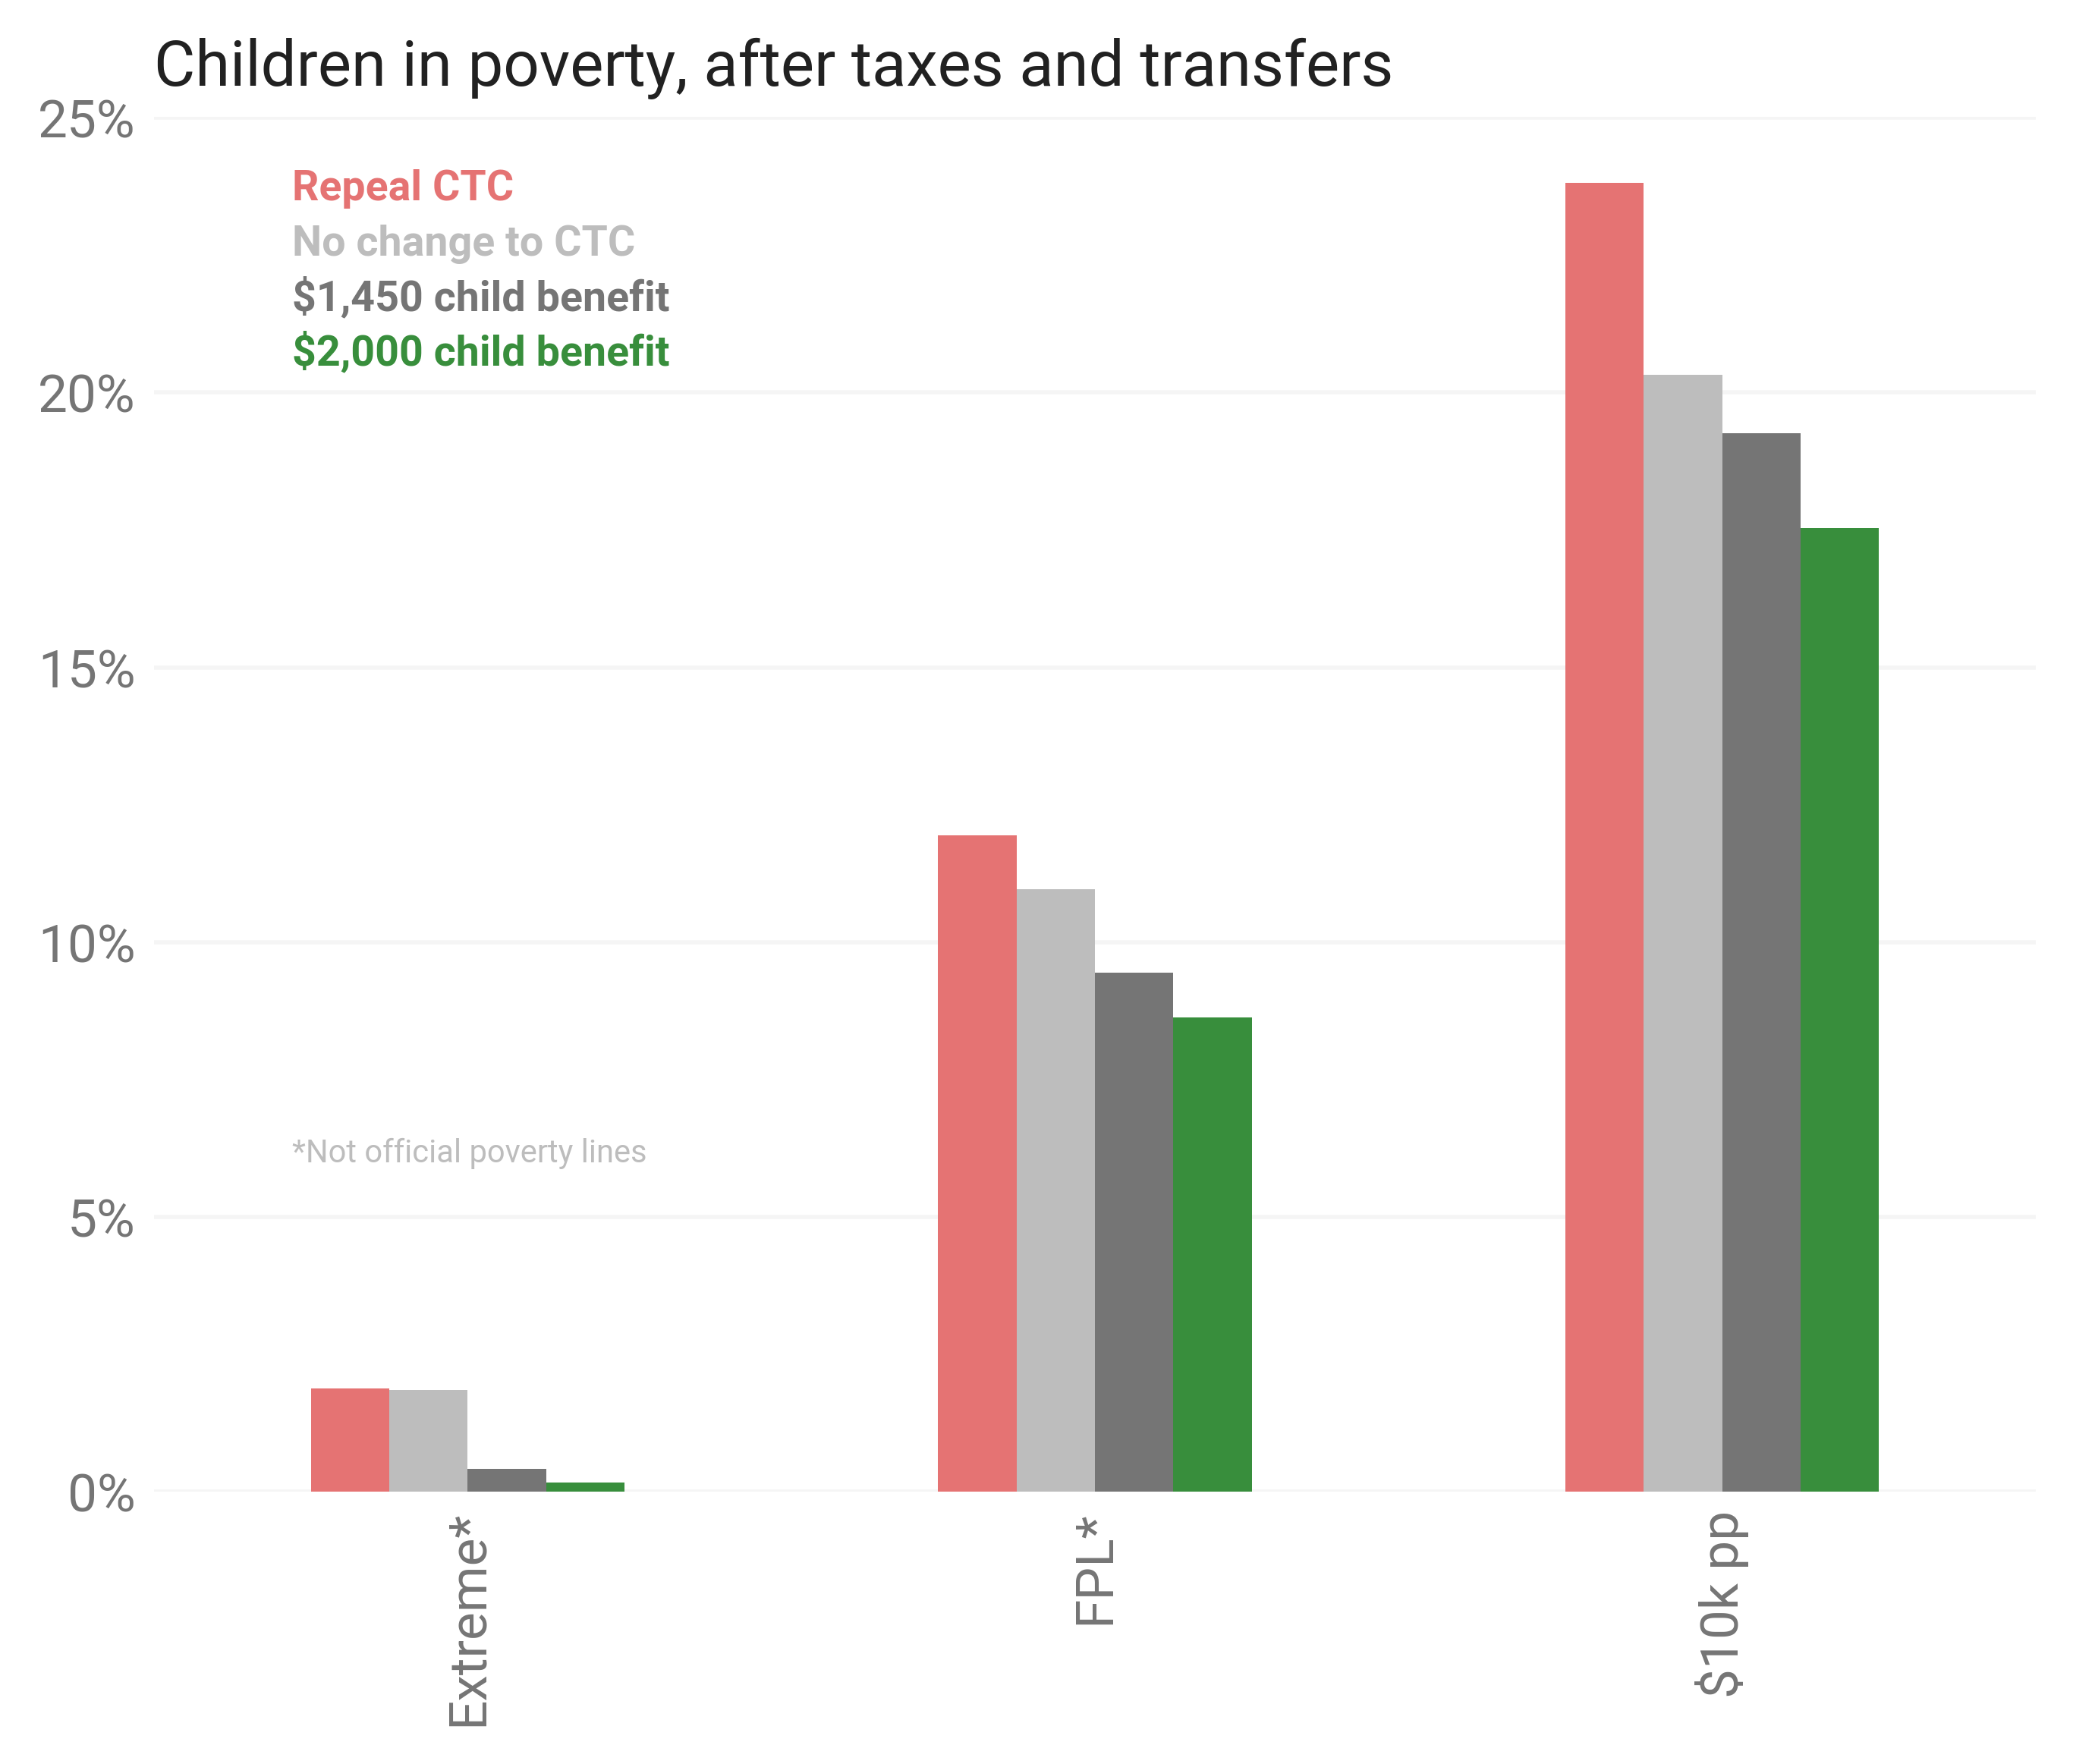
\includegraphics[width=15cm]{poverty.png}
\captionof{figure}{}
\label{fig:poverty}
\end{center}

\section{Discussion} \label{sec:discussion}

This analysis shows that a universal child benefit would be more progressive than the current CTC. Potential follow-ups include alternative metrics and slicing, revisiting with different data, varying the child benefit's structure, and simultaneously altering or removing other programs and tax structures.

Other metrics for poverty and inequality, other units of measurement, other slices, and other types of metrics could paint a more complete picture of a child benefit's impact. A true SPM could be possible with some imputation and would offer consistency with other sources. Inequality measures like "top 1 percent share" and measuring by household or by person rather than tax units would align with analysis groups like the OECD and Congressional Budget Office \cite{burtless2016alternative}. \citeA{bitler2018cash} finds similar distributional effects within groups of filer marital status and racial or ethnic identity, and we may be interested in whether that holds for this reform. Finally, plotting the effect on marginal tax rates would suggest a predicted effect on work incentives.

The amount of a revenue-neutral child benefit varies by up to 16 percent across data sources. When using the PUF instead of CPS data, this analysis yields smaller gains for the bottom quartile, smaller inequality reductions, and higher overall poverty rates (though similar effects of the plan on poverty). Incorporating administrative totals for number of children and CTC outlays into the Tax-Calculator weighting procedure would improve estimates, and resampling would enable variability quantification. More work remains to understand and reconcile differences and improve confidence in results.

Other variants of the child benefit offer their own benefits and drawbacks. Varying the amount depending on child age and number of children may reflect variance in some expenditures like daycare \cite{shaefer2018universal}, but also makes the benefit less comprehensible for beneficiaries. Taxing the benefit and raising the base amount accordingly would further reduce poverty and inequality, but would create administrative challenges if distributing the payment monthly. If taxes are withheld, income would have to be estimated throughout the year; if not withheld, recipients would owe taxes each year, which could be considerable particularly for families with multiple children.

As \citeA{bitler2018cash} and \citeA{hammond2016toward} note, several programs beyond the CTC could fund a more generous revenue-neutral child benefit, especially the child portions of the EITC and nutrition assistance programs. However, because these programs are more targeted to low-income households than the current CTC is, revenue-neutral replacement will leave current beneficiaries worse off. Personal income tax increases could raise revenue from higher earners to mitigate this effect, and in the context of the plan laid out in this article, could also reduce the child benefit's gain for very high earners currently ineligible for the CTC.


\section{Conclusion} \label{sec:conclusion}

By filling the CTC's gap for the lowest-income families, a universal child benefit would reduce inequality and child poverty, effectively eliminating extreme child poverty. A revenue-neutral plan would amount to an income transfer primarily from the upper 70 percent to the bottom 30 percent, while a \$2,000 benefit would avoid net losses and cost either \$27 or \$46 billion, depending on the data source. The TCJA's expansion of the CTC reduces the net losses involved in a revenue-neutral plan, or the cost of topping up to \$2,000 per child.

A child benefit would align the US's child assistance strategy with many European countries, and promote positive child outcomes by investing in proven cash transfers. Its flat amount is easier to transform into a monthly payment, absorbing intra-year income volatility for the poorest families.


% move these to background
By setting a precedent of universalism, a child benefit could become a platform to avoid common issues with arrays of means-tested programs: administrative overhead, abuse by politicians, tensions between recipients and nonrecipients \cite{desai2017rethinking}, and welfare cliffs (implicit marginal tax rates exceeding 100 percent \cite{senate2012cliff}). Replacing the CTC with a child benefit both addresses immediate priorities of reducing poverty and inequality, and puts promotes strategic goals of a more efficient and effective safety net.


\clearpage

\singlespacing
%\setlength\bibsep{0pt}
\bibliographystyle{apacite} % We choose the "plain" reference style.
\bibliography{refs} % Entries are in the "refs.bib" file.

\end{document}